%% beamer:
\documentclass[t, compress]{beamer}

\input{../../base/OptionsListingC++.sty}
\input{../../base/BeamerPackage.sty}

\usepackage{comment}
\usepackage{animate}
\usepackage{tabularx}
\usepackage{booktabs}
\usepackage{colortbl}
\usepackage{tikz}
\usetikzlibrary{calc}
\usepackage[absolute,overlay]{textpos}

\pgfdeclarelayer{background}
\pgfdeclarelayer{foreground}
\pgfsetlayers{background,main,foreground}

\hypersetup{
  backref,
  pagebackref,
  naturalnames=true,
  colorlinks=true,
  urlbordercolor={0.0 0.2823 0.43921},
  urlcolor=upsud_blue
}

%% document infos:
\title{\textbf{Présentation des projets \Cpp}}

\subtitle{}

\author[Présentation des projets]{}

\date[]{}

%% document:
\begin{document}

\frame[c, plain]{\titlepage}

\begin{frame}[c, fragile]{Organisation du second semestre}

  \begin{center}
    \begin{tikzpicture}
      \node (tbl) {
        \begin{tabularx}{\textwidth}{rXr}
          \arrayrulecolor{upsud_blue}
          \structure{Aujourd'hui} & \textcolor{upsud_blue}{Présentation des sujets}\rule{0pt}{2.5ex} \\[2ex]
          \textcolor{upsud_blue}{9 -- 14 Janvier} &  \textcolor{upsud_blue}{Indication aux enseignants du projet choisi (via formulaire web)}\\[2ex]
          \textcolor{upsud_blue}{11 -- 15 Mars} &
          \textcolor{upsud_blue}{Remise des programmes \textbf{par
              mail} à \href{xavier.garrido@u-psud.fr}{\ding{41}~xavier.garrido@u-psud.fr}} \\[2ex]
          \textcolor{upsud_blue}{18 Mars avant 16h} &  \textcolor{upsud_blue}{Remise des rapports au Secrétariat} \\[2ex]
          \textcolor{upsud_blue}{19 Mars à 12h} &  \textcolor{upsud_blue}{Affichage des plannings de soutenances} \\[2ex]
          \textcolor{upsud_blue}{19 -- 26 Mars} &  \textcolor{upsud_blue}{Soutenances de projet informatique}\\[2ex]
      \end{tabularx}};
      \begin{pgfonlayer}{background}
        \draw[rounded corners, top color=upsud_blue!20,draw=white]
        ($(tbl.north east)-(0.0,0.0)$) rectangle ($(tbl.south west)+(0.13,0.2)$);
      \end{pgfonlayer}
    \end{tikzpicture}
  \end{center}

\end{frame}

\begin{frame}[c, fragile]{Présentation des projets}

  %% Projets du Lundi (P. Fromy)

  %% \begin{itemize}

  %% \item \'Equation de la chaleur
  %% \item Résolution d'équations intégrales
  %% \item Atome d'hélium
  %% \item \'Etat d'équilibre thermique d'une plaque
  %% \item Modèle de Thomas-Fermi
  %% \item Estimation d'une intégrale par la méthode de Monte-Carlo

  %% \end{itemize}

  %% Projets du Mercredi

  \begin{itemize}

  \item \structure{Méthode d'optimisation : le recuit simulé}
  \item \structure{L'Observatoire Pierre Auger}
  \item Le jeu d'échec
  \item Traitement d'images

  \end{itemize}

\end{frame}

\begin{frame}[c, fragile]{Méthode d'optimisation : le recuit simulé}

  \begin{itemize}
  \item Historiquement, le nom et l'inspiration proviennent du récuit en
    métallurgie
  \end{itemize}

  \begin{center}
      \includegraphics[scale=0.5]{figures/heat-0}
  \end{center}

\end{frame}

\begin{frame}[c, fragile]{Méthode d'optimisation : le recuit simulé}

  \begin{itemize}
  \item Historiquement, le nom et l'inspiration proviennent du récuit en
    métallurgie
  \item Physiquement, le mécanisme naturel de minimisation de
    l'énergie repose sur la distribution de probabilité de Boltzmann


    \begin{equation*}
      \structure{p\,(E\,)\propto\exp\left(-\frac{\Delta E}{kT}\right)}
    \end{equation*}

  \end{itemize}

\end{frame}


\begin{frame}[c, fragile]{Méthode d'optimisation : le recuit simulé}

  \begin{itemize}

  \item Mathématiquement, le recuit simulé est un algorithme
    d'optimisation i.e. de recherche de minima d'une fonction donnée

    \begin{center}
      \includegraphics[scale=0.5]{figures/sam_0}
    \end{center}

  \end{itemize}

\end{frame}

\begin{frame}[c, fragile]{Méthode d'optimisation : le recuit simulé}

  \begin{itemize}

  \item Mathématiquement, le recuit simulé est un algorithme
    d'optimisation i.e. de recherche de minima d'une fonction donnée

    \begin{center}
      \includegraphics[scale=0.5]{figures/sam_1}
    \end{center}

  \end{itemize}

\end{frame}

\begin{frame}[c, fragile]{Méthode d'optimisation : le recuit simulé}

  \begin{itemize}

  \item Mathématiquement, le recuit simulé est un algorithme
    d'optimisation i.e. de recherche de minima d'une fonction donnée

    \begin{center}
      \includegraphics[scale=0.5]{figures/sam_2}
    \end{center}

  \end{itemize}

\end{frame}

\begin{frame}[c, fragile]{Méthode d'optimisation : le recuit simulé}

  \begin{itemize}

  \item Mathématiquement, le recuit simulé est un algorithme
    d'optimisation i.e. de recherche de minima d'une fonction donnée

    \begin{center}
      \includegraphics[scale=0.5]{figures/sam_3}
    \end{center}

  \end{itemize}

\end{frame}

\begin{frame}[c, fragile]{Méthode d'optimisation : le recuit simulé}

  \begin{itemize}

  \item Mathématiquement, le recuit simulé est un algorithme
    d'optimisation i.e. de recherche de minima d'une fonction donnée

  \item Domaine d'application : problème multi-variables

    \begin{itemize}

    \item informatique,
    \item génétique,
    \item physique ...

    \end{itemize}

  \end{itemize}

\end{frame}

\begin{frame}[c, fragile]{Objectifs du projet}

  \begin{itemize}

  \item Régression linéaire, parabolique, études en fonction de
    l'incertitude sur les données expérimentales~\ldots

  \item Résolution du problème du voyageur de commerce
    \begin{block}{}
      \centering
      \href{http://www-i1.informatik.rwth-aachen.de/~algorithmus/algo41.php}{http://www-i1.informatik.rwth-aachen.de/...} \\
      \href{http://interstices.info/jcms/c_43811/le-recuit-simule}{http://interstices.info/...}
    \end{block}

  \end{itemize}

\end{frame}

{
\usebackgroundtemplate{
  \includegraphics[width=\paperwidth]{figures/auger-0}
}

\setbeamertemplate{footline}[default]

\begin{frame}[c, fragile]{\colorbox{white}{L'Observatoire Pierre Auger}}

  \begin{textblock}{5}(0.5,12.5)
    \begin{beamerboxesrounded}[upper=lbtuc,lower=lbtuc,shadow=false]
      {}\vspace{-0.1cm}
      \begin{center}
        \scriptsize L'Observatoire Pierre Auger est situé à Malargüe
        (Argentine) et est \textbf{le premier détecteur hybride} construit
        sur une surface de \textbf{\unit[3000]{km$^2$}}
      \end{center}
    \end{beamerboxesrounded}
  \end{textblock}

\end{frame}

\begin{frame}[c, fragile]{\colorbox{white}{L'Observatoire Pierre Auger}}

  \begin{textblock}{5}(4,6.6)
  \begin{tikzpicture}
    \node[rectangle,
      color=upsud_red,fill=upsud_red,fill opacity=0.3,
      line width=1.5pt,
      draw, rounded corners,
      text width=0.5cm,
      text height=0.5cm] {};
  \end{tikzpicture}
  \end{textblock}
  \begin{textblock}{5}(5.55,11.6)
    \begin{tikzpicture}
      \node[rectangle,
        color=upsud_red,fill=upsud_red,fill opacity=0.3,
        line width=1.5pt,
        draw, rounded corners,
        text width=0.5cm,
        text height=0.5cm] {};
    \end{tikzpicture}
  \end{textblock}
  \begin{textblock}{5}(12.4,10.3)
    \begin{tikzpicture}
      \node[rectangle,
        color=upsud_red,fill=upsud_red,fill opacity=0.3,
        line width=1.5pt,
        draw, rounded corners,
        text width=0.5cm,
        text height=0.5cm] {};
    \end{tikzpicture}
  \end{textblock}
  \begin{textblock}{5}(10.2,5.7)
    \begin{tikzpicture}
      \node[rectangle,
        color=upsud_red,fill=upsud_red,fill opacity=0.3,
        line width=1.5pt,
        draw, rounded corners,
        text width=0.5cm,
        text height=0.5cm] {};
    \end{tikzpicture}
  \end{textblock}

  \begin{textblock}{5}(4.5,2.5)
    \begin{beamerboxesrounded}[upper=lrtuc,lower=lrtuc,shadow=false]
      {}\vspace{-0.1cm}
      \begin{center}
        \scriptsize \textbf{24 télescopes de fluorescence}
        détectant la lumière de désexcitation du N$_2$
        (\unit[300-400]{nm}) émise au passage des $e^\pm$ de la
        gerbe \\ \textbf{$\rightarrow$ profil longitudinal}
      \end{center}
    \end{beamerboxesrounded}
  \end{textblock}

\end{frame}

\begin{frame}[c, fragile]{\colorbox{white}{L'Observatoire Pierre Auger}}

  \begin{textblock}{5}(4.5,2.5)
    \begin{beamerboxesrounded}[upper=lrtuc,lower=lrtuc,shadow=false]
      {}\vspace{-0.1cm}
      \begin{center}
        \scriptsize \textbf{24 télescopes de fluorescence}
        détectant la lumière de désexcitation du N$_2$
        (\unit[300-400]{nm}) émise au passage des $e^\pm$ de la
        gerbe \\ \textbf{$\rightarrow$ profil longitudinal}
      \end{center}
    \end{beamerboxesrounded}
  \end{textblock}
  \begin{textblock}{6}(3,10.5)
    \begin{beamerboxesrounded}[upper=lrtuc,lower=lrtuc,shadow=false]
      {}\vspace{-0.1cm}
      \begin{center}
        \scriptsize \textbf{1600 cuves d'eau} placées à
        \unit[1500]{m} les unes des autres et chargées de détecter les
        particules secondaires via \textbf{la production de lumière
          Cherenkov} \\ \textbf{$\rightarrow$ profil latéral}
      \end{center}
    \end{beamerboxesrounded}
  \end{textblock}

\end{frame}
}

\begin{frame}[c, fragile]{L'Observatoire Pierre Auger}

  \vspace{-2cm}
  \includegraphics[width=0.9\paperwidth]{figures/AugerEvent-1}

\end{frame}

\begin{frame}[c, fragile]{L'Observatoire Pierre Auger}

  \begin{textblock}{6}(1,3)
    \includegraphics[scale=0.25]{figures/AugerEvent-1}
  \end{textblock}

  \begin{textblock}{6}(8,0.5)
    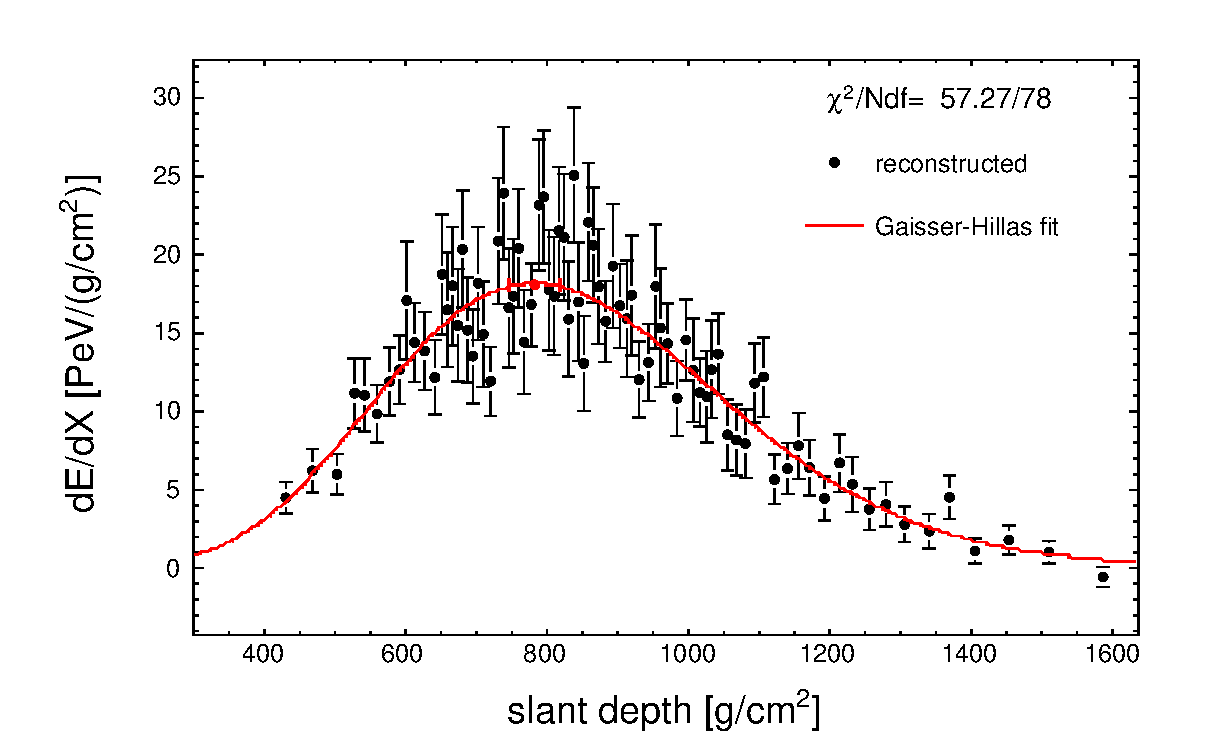
\includegraphics[scale=0.32]{figures/gh}\\
    \includegraphics[scale=0.32]{figures/ldf}
  \end{textblock}

\end{frame}

\begin{frame}[c, fragile]{Objectifs du projet}

  \begin{itemize}

  \item 2 projets de simulation/reconstruction de gerbes
    atmo. :

    \begin{enumerate}

    \item Reconstruction latérale du signal (SD)

    \item Reconstruction longitudinale (FD)

    \end{enumerate}

  \end{itemize}

\end{frame}

\begin{frame}[c, fragile]{Présentation des projets}

  \begin{itemize}

  \item \structure{Méthode d'optimisation : le recuit simulé}
  \item \structure{L'Observatoire Pierre Auger}
  \item Le jeu d'échec
  \item \textbf{\structure{Traitement d'images $\rightarrow$ présentation
    lundi prochain}}
  \end{itemize}

\end{frame}


\end{document}

% Local Variables:
% mode: latex
% coding: utf-8-unix
% End:
